\section{Introduction}

The objective of process control is to keep key process-operating parameters within narrow bounds of the reference value or setpoint. Controllers are used to automate a human function in an effort to control a variable. A basic controller can keep an individual loop on an even point, so long as there is not too much disruption. Complex processes like ones in metallurgy might employ dozens or even hundreds of such controllers, but keeping an eye on the big picture was, until not so long ago, a human process.

Although a device was used to automate a human function in an effort to control a variable, there was no sense of what the process was doing overall. A basic controller could keep an individual loop on an even keel, more or less, so long as there was not too much disruption. Complex processes might employ dozens or even hundreds of such controllers, each with its performance displayed on a panel board, but keeping an eye on the big picture was still a human process.

When distributed control system (DCS) platforms were introduced in the 1970s, they simplified the mechanics of the panel board, but did not do much to improve its capabilities. Big-picture analysis was still largely a human responsibility. Sure, getting beyond the technical constraints of pneumatic field devices with their troublesome compressed air tubing made it easier to install more instruments and actuators, but the basic control concepts did not really change. Any movement to advanced process control (APC) and other forms of control optimization were still in their infancy. Process automation capable of supporting APC had to encompass many technologies and techniques. It was characterized by incorporating many more input data points into algorithms and orchestrating more complex sequences.

The transition to process automation and advanced process control (APC) was empowered by being able to create an all-encompassing platform capable of coordinating more than single loops or small cascade groups. One major advantage of newer platforms is the ability to optimize a process to suit the owner’s specific economic goals based on any number of desired outcomes. The process automation system can operate the plant to minimize energy consumption, maximize output, and deliver specific product quality attributes.

Implementing such systems is challenging. During the initial design phase of a control system upgrade or a new installation, it is far too easy to focus just on process fundamentals, and never get beyond considering desired steady-state conditions. Automation system upgrades and new installations can therefore miss opportunities to engage with process and automation technology experts capable of uncovering better ways of doing things. Many capabilities of modern process automation systems are still underutilized in most process plants. Far fewer companies use APC as effectively as they could, even though basic APC technologies have been around for decades.

Modeling, together with simulation, are important parts of engineering. Integrating them into engineer's toolbelt yields many benefits. Before actual testing in physical reality, one can do many different virtual tests by simulating the modeled phenomena with lower overhead of financial requirements. There's also close to zero risk of hurting anybody (most notable risk being ill-treatment of electricity). Still, coming up with and refining actual mathematical or physical model, to the point of it being accurate enough for the job at hand, takes a lot of time. Also, actual simulation part can take hours or days to converge. However, it can be argued that, in some industrial applications, broad parameter space mapping is sometimes more valuable than higher order analysis of fewer design points \citep{harwoodREALTIMEMODELLINGSIMULATION}.

With the continuation of expanding computational power available for engineers that can tap into it for their simulations, the time for simulation to converge decreases accordingly. it becomes clear enough that ...

We'll discuss the path towards interactive simulation in section \ref{interactive-simulation}.


\section{Modeling and Simulation}

\begin{chapquote}{R. W. Hamming, \textit{The Art of Doing Science and Engineering}}
``The purpose of computing is insight, not numbers"
\end{chapquote}

Why simulation?

Investigate what cannot be measured

Reduce need for testing

Design optimization: narrow design space

Proactive instead of reactionary design

\subsection{Mathematical Modeling}

\subsection{Numerical Simulation}

%-- prepisat (zdroj https://www.nature.com/subjects/numerical-simulations)
A numerical simulation is a calculation that is run on a computer following a program that implements a mathematical model for a physical system. Numerical simulations are required to study the behaviour of systems whose mathematical models are too complex to provide analytical solutions, as in most nonlinear systems.
%------

% prepisat
The motivation for using computer simulations to investigate complex processes is two-fold. , it enables design changes to be tested before building a prototype, which naturally leads to a lower total design cost. Second, it makes it possible to investigate phenomena that cannot easily be measured or observed in the process. Even a seemingly simple operation such as the continuous measurement of the temperature during the decarburization process is difficult due to the very high temperatures in the process and generally harsh conditions prevailing in the steel plants
%---

\subsection{Computational Fluid Dynamics}

% --- Prepisat -------------------
Modern fluid mechanics problems would be impossible to solve without use of Computational Fluid Dynamics (CFD), since the scope of analytical solutions to fundamental equations of fluid mechanics is very limited and, once a more difficult geometry is encountered, we usually have to choose a given numerical method for obtaining a solution. CFD encompasses a wide spectrum of numerical methods used for solving complex three-dimensional (3D) and time-dependent flow problems (Rapp; 2017). Since early pioneering work in the metallurgical field done by Szekely et al. (1977), the cost of performing computer simulations has decreased over the last few decades, while the available processing power has increased. Most of the processors and processing units that are currently developed and produced have several cores that can execute instructions in parallel. Thus, the processing power available to a CFD software also depends on the capability of the software to execute in parallel. A study by Ersson and Tilliander (2018) of the last two decades of metallurgical CFD simulations reveals huge improvements on the type of phenomena that can be explored and we will see this trend is continuing thanks to improvements in both the available processing power and the avail- able algorithms. Therefore CFD found its way into numerous studies in steelmaking, where these methods proved useful in demonstrating the hidden and significant proper- ties. However, its use in the steel industry may not be as integrated as in the aero and automotive industries, in which the development of new designs is of key importance. The major difference between aero and metallurgical industries is that the metallurgical industries almost always deal with multiphase systems at elevated temperatures and that the motivation of modeling is mainly process optimization. With a continuing development in multiphase models as well as in reacting flow modeling, the continued usefulness of CFD in metallurgy remains clear.
% --------------------------------------------------

\subsection{Integrated Modeling and Simulation}


% --- Prepisat -------------------
%The motivation for using computer simulations to investigate metallurgical processes is two-fold. First, it enables design changes to be tested before building a prototype, which naturally leads to a lower total design cost. Second, it makes it possible to investigate phenomena that cannot easily be measured or observed in the process. Even a seemingly simple operation such as the continuous measurement of the temperature during the decarburization process is difficult due to the very high temperatures in the process and generally harsh conditions prevailing in the steel plants (Ersson and Tilliander; 2018).
% -----------------------------

% --- Prepisat -------------------
%In metallurgy, simulating linear and non-linear processes that we encounter in steelmaking by creating mathematical models is of great importance. Since first attempts to use mathematical techniques for the simulation and optimization of large scale metallurgical operations (Ray et al.; 1973), various numerical methods were implemented as algorithms and used to simulate phenomena in steelmaking processes. One class of such methods is Monte Carlo, which is useful for simulating systems with many coupled degrees of freedom such as fluids.
% -------------------------------------------


% --- Prepisat -------------------
%In LD/BOF process, different chemical reactions among oxygen, slag, and molten iron in oxygen converter, in combination with vigorous stirring process to promote slagging, dephosphorization, decarbonization, heating of molten steel, and homogenization of steel composition and temperature, determines the final properties of steel. The objective of the oxygen converter is to refine molten iron to crude steel through oxidization to achieve a specified temperature and chemical composition at the end blow. Failure to do this leads to the need to reblow. The impact of oxygen jet into molten bath strongly affects the bath and promotes the three-phase flow among gas, slag, and molten steel in the bath. With the move from old rule-based systems to a model-based, real-time closed-loop control of lance movement and oxygen flow, significant drawbacks were eliminated. There have been efforts in developing accurate and efficient numerical models within CFD field to solve the jets flow in the oxygen converter. Peng and Han (1996) established the conditions of optimum nozzles of performance by deriving the system of mathematical equations to simulate the steady, quasi-one-dimensional supersonic flow through a sin- gle De Laval nozzle. Tago and Higuchi (2003) analyzed single-nozzle and multi-nozzle lances with the help of two-dimensional simulation based on fluid dynamics and found that higher ambient temperature leads to the lower density and the higher velocity of the gas jets, but does little affect the dynamic pressure. They report that CFD proved use- ful method to predict the effect of the inclination angle and the number of the nozzles on the jet behavior in the top blown processes. Wang, Yuan, Matsuura, Zhao, Cheng and Tsukihashi (2010) developed a three-dimensional mathematical model to simulate the compressible jets flow from the top-blown lance, taking into consideration variations of fluid density, viscosity, high temperature and Mach number. They demonstrated that $k–\omega$ turbulence model is superior to the widely used $k–\epsilon$ turbulence model to calculate turbulent conditions within multiple jets.
% -------------------------------

% --- Prepisat -------------------
%CFD models have been also used in developing deeper understanding of the decarburization processes in steelmaking. However, these processes are highly complex with large variations in time and length, and therefore it makes the systems extremely demanding to simulate. Ersson and Tilliander (2018) reviewed latest research on the subject from 1998 until 2016 and found out that, even though several reports have been published dis- cussing research about modeling parts of the decarburization processes numerically, no models have been presented that can handle the entire complexity of the processes. Many authors had simplified the system in existing models in order to achieve an understanding of particular phenomena rather than of the entire process.
% -----------------------------------------

% --- Prepisat -------------------
%Another important part of the oxygen steelmaking process is keeping the usual balance of $80\%$ hot metal and $20\%$ scrap during charging to regulate the temperature of steel in the vessel. To define the charge conditions and oxygen blowing requirements to achieve the temperature and chemical composition, mathematical and thermodynamic models have been developed \citep{Kacur2019, sprava2017}. Reactions that take place in LD process can vary significantly from heat to heat, while not many variables involved are not accurately known. Therefore, it is necessary to take into account the uncertainty affecting the whole process reactions. To correct the differences between the theoretical predictions of the process models and the real results, Bouhouche et al. (2012) introduced a random quantity term into their models and improved the prediction model with the use of Support Vector Regression and Monte Carlo Simulation methods in combination. Most of the control schemes rely on an accurate system model. However, as these systems become more complex, writing down the dynamics from the first principles is extremely challenging. In such cases, neural networks are used to approximate the dynamics directly using system data. In this context, neural networks can be thought of as a generalization of linear regression for non-linear dynamics. At the Institute of Control and Informatization of Production Processes at BERG Faculty (TUKE), team around Laciak et al. (2018) built upon Bouhouche’s work and started experimenting with machine learning in pro- cess control and its application in oxygen steelmaking, precisely in LD converter. They applied Support Vector Machines (SVM) and Support Vector Regression (SVR) to predict the final melt temperature and final carbon concentration based on dynamical data. Their work also focuses on developing innovative fractional-order mathematical models for indirect measurement of molten steel temperature and concentration of CO and CO2. The non-linear nature of these processes presents the opportunity to model them by using derivatives of non-integer order, which in their definition are based on the influence of past data on the present value of derivative.
% --------------------------------------

\section{Lattice Boltzmann Method}

LBM	formulated in 1988 by	McNamara and	Zanetti

– 1859:	Maxwell's	distribution	function	

– 1868:	Boltzmann	transport	equation	

– 1954:	Bhatnagar,	Gross,	and	Krook	(BGK)	collision	operator	

– 1956:	FEM	by	Turner	

– 1973,76:	Hardy,	Pomeau,	and	de	Pazzis	(HPP)	model/Lattice	
Gas	Automata	(LGA)	

– 1980:	Finite	volume	method	(FVM)	at	Imperial	College	

%% --- Prepisat -------------------
LB method has witnessed an astonishing growth in its methodology development and application over the past quarter of a century. It fills a vital gap between the macroscopic continuum approaches such as the Navier–Stokes solvers and the particle-based microscopic approaches such as molecular dynamics. Such a mesoscopic approach has found applications in almost all areas of energy and combustion \cite{liLatticeBoltzmannMethods2016a}.
% -------------------------------------

The lattice Boltzmann method (LBM) originally grew out of the lattice gas automata \cite{succi2001lattice}. It is positioned in the middle between Eulerian and Lagrangian methods for solving fluid flow problems. Instead of calculating the properties of individual particles, the particle distribution function (PDF) is used for describing the distribution of particles that is computed for each node in the discretized domain. As we mentioned earlier, each node needs only its neighbours for the actual computation, allowing for good parallelization. A collision of particle distributions is described by $\Omega$ operator, that states the rate of change of PDF (denoted as $f$) is equal to the rate of collision in the limit of $dt \xrightarrow[]{} 0$:

\begin{equation}
	\label{eq:collision-operator}
	\frac{df}{dt} = \Omega(f).
\end{equation}

The collision operator $\Omega$ is difficult to solve. It's been simplified by the work of Bhatnagar, Gross and Crook \cite{bhatnagarModelCollisionProcesses1954}, that introduced the BGK operator

\begin{equation}
	\label{eq:bgk-operator}
	\Omega_i = \frac{1}{\tau}(f^{eq}_i - f_i),
\end{equation}
where $f^{eq}_i $ is an particle distribution function in an equilibrium state of the system obtained by Taylor expansion of the Maxwell-Boltzmann equilibrium function. The relaxation parameter $\tau$ is the reciprocal that presents a time in which the systems relaxes towards the equilibrium.

The Lattice Boltzmann Equation (LBE) in its discrete form, the fundamental part of the lattice Boltzmann method, is obtained by discretization of the velocity space of the Boltzmann equation into a finite number of discrete velocities $e_i$, $i = 0,1,...,8$. It can be stated as

\begin{equation}
	\label{eq:lbe-bgk}
	f_i (\bm{x}+\bm{e}_i\Delta t,t+\Delta t) = f_i (\bm{x},t)-\frac{1}{\tau}\Big[f_i (\bm{x},t) - f_i^{eq} (\bm{x},t)\Big],
\end{equation}
where $f_i (\bm{x},t)$ denotes the individual direction of the PDF at each lattice point in particular time and $f_i (\bm{x}+\bm{e}_i\Delta t,t+\Delta t)$ is equal to resulting PDF for all neighbouring nodes in the next iteration step. Necessary criterion for stability is that physical information should not travel faster than fastest speed supported by the lattice \cite{succi2001lattice}.

Macroscopic quantities are obtained from hydrodynamic moments of the distribution function. They are computed with \ref{eq:density} and momentum flux \ref{eq:velocity} (from which the velocity can be obtained by simply dividing the equation by $\rho$)

\begin{equation}
	\label{eq:density}
	\rho = \sum_{i=0}^{9}f_i,
\end{equation}

\begin{equation}
	\label{eq:velocity}
	\rho\bm{u} = \sum_{i=0}^{9} \bm{e}_i  f_i .
\end{equation}

Equilibrium distribution function $f^{eq}$ can be expressed by performing a Hermite expansion of the Boltzmann equilibrium function as

\begin{equation}
	\label{eq:feq}
	f_i^{eq} = \omega_i \rho \left( 1+3\frac{\bm{e}_i \cdot \bm{u}}{c_s} + \frac{9}{2}\frac{(\bm{e}_i \cdot \bm{u})^2}{c_s^2}-\frac{3}{2}\frac{\bm{u}^2}{c_s^2}\right),
\end{equation}
where $c_s$ is the speed of sound within the lattice, usually set to $c_s = \frac{1}{\sqrt{3}}$ and $\omega$ denotes different weights for discrete velocity in D2Q9 stencil

\begin{align}
	\label{weights}
	\omega_0 &= 4/9,\\
	\omega_{1,2,3,4} &= 1/9,\\
	\omega_{5,6,7,8} &= 1/36.\\
\end{align}

With a proper set of discrete velocities, the LBE recovers the incompressible Navier–Stokes equations by the Chapman–Enskog expansion. For the flows within the incompressible limit, assumptions such as low-Mach number and variations in density of order $\mathcal{O}(M^2)$ has to be made.

The present study focuses on the D2Q9 discrete velocity model which is illustrated in Fig. \ref{fig:d2q9-node}. 

\begin{figure}[!ht]
	\centering
	\captionsetup{justification=centering}
	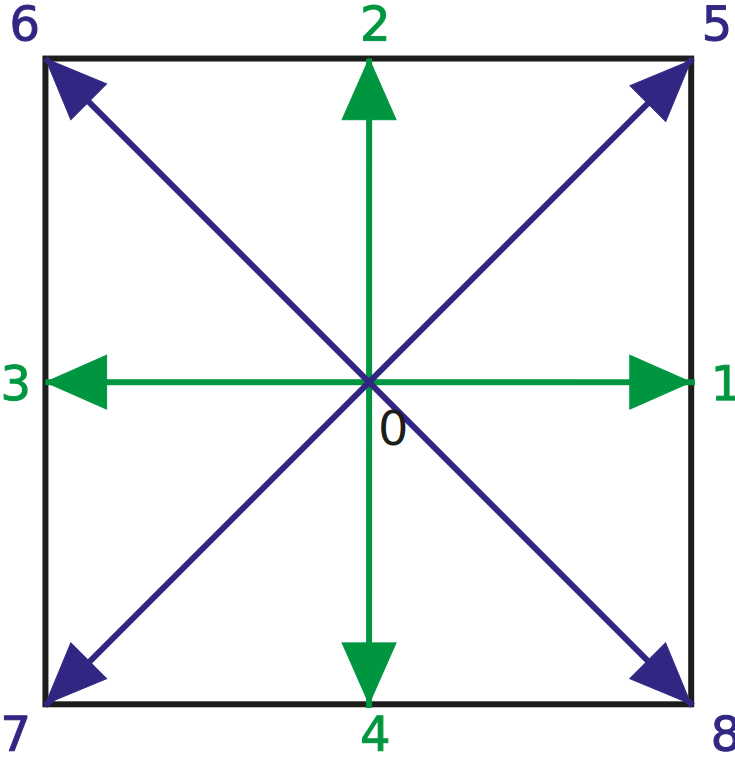
\includegraphics[width=0.25\textwidth]{figures/D2Q9_colored.pdf}
	\caption{D2Q9 lattice node scheme.}
	\label{fig:d2q9-node}
\end{figure}

Discrete velocities $\bm{e}_i$ are expressed as

\begin{equation}
	\label{discrete-velocities}
	\bm{e}_i = \begin{bmatrix}
		0 & 1 & 0 &-1 & 0 & 1 &-1 &-1 & 1\\
		0 & 0 & 1 & 0 &-1 & 1 & 1 &-1 &-1
	\end{bmatrix}
\end{equation}

Two general steps of the LBM solver involve solving  Eq. \ref{eq:collision} for collision and Eq. \ref{eq:streaming} for streaming in each iteration.

\begin{equation}
	\label{eq:collision}
	f_i (\bm{x},t+\Delta t) = f_i (\bm{x},t)-\frac{1}{\tau}\Big[f_i (\bm{x},t) - f_i^{eq} (\bm{x},t)\Big].
\end{equation}

\begin{equation}
	\label{eq:streaming}
	f_i (\bm{x}+\bm{e}_i\Delta t,t+\Delta t) = f_i (\bm{x},t+\Delta t).
\end{equation}

For the boundary condition, we implemented a simple no-slip boundary known as bounce-back, which effectively reverses the direction of $f_i$ \cite{Mawson2014InteractiveFI}. In places like input and output of simulated pipe for Kármán vortex test case, we implemented periodic boundary conditions \cite{succi2018lattice}.

% --- Prepisat -------------------
During the last three decades, the mesoscopic lattice Boltzmann method (LBM), based on the kinetic theory, has become an increasingly important method for numerical simulations of multiphase flows, mainly on account of its meso-scale features, easy the numerical stability compared with the SRT-LBM. The corresponding non-orthogonal MRT-LBM has been extended to sim 
% ----------------------------


\subsection{Kinetic Theory}

The main properties of any numerical scheme can be classified as follows \citep{succi2001lattice}:

\begin{itemize}
	\item causality,
	\item accuracy,
	\item stability,
	\item consistency,
	\item efficiency,
	\item flexibility. 
\end{itemize}

With respect to above properties, lattice Boltzmann equation (LBE) can be classified as an explicit, Lagrangian, finite-hyperbolicity approximation of Navier-Stokes equations. 


The LBE is obtained by discretizing the velocity space of the Boltzmann equation into a finite number of discrete velocities $e_\alpha$ \{$\alpha$ = 0,1,...,26\}. With a proper set of discrete velocities, the LBE recovers the continuum Navier–Stokes equations by the Chapman–Enskog expansion.


\begin{figure}[!ht]
	\centering
	\subfloat[D3Q19]{{\includegraphics[width=6cm]{figures/d3q19.jpg} }}
	\qquad
	\subfloat[D3Q27]{{\includegraphics[width=6cm]{figures/d3q27.jpg} }}
	\caption{Three-dimensional lattice node schemes.}
	\label{fig:lattice-node-schemes}
\end{figure}


Caution have to be taken when working within lattice's discrete world. For simulating the interface of blown oxygen with melted fluid slag, we're working with higher Mach speeds. The basic notion is that the lattice can only support signals with a finite propagation speed. Necessary criterion for stability is that physical information should not travel faster than fastest speed supported by the lattice \cite{succi2001lattice}.

We can calculate the error to $\varepsilon(Ma^3)$ in space and proportional to $\varepsilon (Ma \cdot dt)$ in time, where $Ma = \frac{u}{c_s}$ is the Mach number of the system.

$p = c_s^2 \rho$ is the pressure, $c_s = \frac{c}{\sqrt{3}}$ is the speed of sound, and the kinematic and viscosity $\nu$ is related to the relaxation time rates for the second-order moments by $\nu = \left(\frac{1}{s_v - 0.5}\right) c_s^2 \Delta t$ and $\xi = \frac{2}{3}\left(\frac{1}{s_b - 0.5}\right)$ respectively.


\subsection{Bhatnagar-Gross-Krook Model}


- TODO: napisat aj o klasickom BGK modeli \citep{bgk1954}

The collision operator $\Omega$ is difficult to solve. It's been simplified by the work of Bhatnagar, Gross and Crook \cite{bhatnagarModelCollisionProcesses1954}, that introduced the BGK operator

\begin{equation}
	\label{eq:std-bgk}
	f_i (\bm{x}+\bm{e}_i\Delta t,t+\Delta t) = f_i (\bm{x},t)-\frac{1}{\tau}\Big(f_i (\bm{x},t) - f_i^{eq} (\bm{x},t)\Big)
\end{equation}

In the presence of a body force density $\bm{F} = \rho \bm{g}$, where $\bm{g}$ is
the acceleration due to $\bm{F}$, the LBE must be modified to account for the force \cite{guoDiscreteLatticeEffects2002}.

\begin{equation}
	\label{eq:feq}
	f_i^{eq} = \omega_i \rho \left( 1+3\frac{\bm{e}_i \cdot \bm{u}}{c} + \frac{9}{2}\frac{(\bm{e}_i \cdot \bm{u})^2}{c^2}-\frac{3}{2}\frac{\bm{u}^2}{c^2}\right)
\end{equation}

\begin{equation}
	\label{eq:density}
	\rho = \sum_{i=0}^{27}f_i
\end{equation}

\begin{equation}
	\label{eq:velocity}
	\rho\bm{u} = \sum_{i=0}^{27} f_i \bm{e}_i + \frac{\Delta t \bm{F}}{2}
\end{equation}

\subsection{Multiple Relaxation Time}

% --- Prepisat -------------------
To overcome difficulties of numerical instability in applying the LBM method, the multiple-relaxation-time (MRT) scheme is useful to stabilize the solution and to obtain satisfactory results because the MRT model allows the usage of an independently optimized relaxation-time for each physical process \cite{sugaD3Q27MultiplerelaxationtimeLattice2015}.
% -----------------------------------------------

A general collision step in MRT can be written as \cite{feiModelingRealisticMultiphase2019}

\begin{equation}
	\label{eq:mrt-collision}
	f_i^{*} (\bm{x},t) = f_i (\bm{x},t)-\Lambda_{i,k}\big[f_k - f_k^{eq}\big]_{(\bm{x},t)} +\frac{\Delta t}{2} \big[ F_i (\bm{x},t) +  F_i (\bm{x}+\bm{e}_i\Delta t,t+\Delta t) \big]
\end{equation}

where $\bm{x}$ is the spatial position in the 3D grid, $t$ is time, $F_i$ are the forcing terms in discrete velocity space, and collision operator $\Lambda_{i,k}$ computed as \cite{feiModelingRealisticMultiphase2019}

Although many schemes to discretize the velocity space have been proposed, for three-dimensional (3-D) flows, the present study focuses on so called the three- dimensional twenty-seven (D3Q27) discrete velocity model which is illustrated in Fig. 1. Table 1 lists the sound speed $c_S$ , the discrete velocity $e_\alpha$ and the weight parameter $w_\alpha$ in the model with $c = \delta x / \delta t$ where $\delta x$ and $\delta t$ are the lattice spacing and the time step, respectively. The MRT LBM transforms the distribution function in the velocity space to the moment space by the transformation matrix $M$ . Transformation matrix $\bm{M}$ can be obtained from Eqs. \ref{eq:moments}.

\begin{equation}
	\label{eq:moments}
	M = ... doplnit
\end{equation}

Since the moments of the distribution function correspond directly to flow quantities, the moment representation allows us to perform the relaxation processes with different relaxation-times according to different time-scales of various physical processes. The evolution equation for the particle distribution function f is thus written as

\begin{equation}
	|f (x_i +e_\alpha \delta t,t+ \delta t)\rangle-|f (x_i,t)\rangle=-M^{-1} S [|m(x_i,t)\rangle - |m^{eq} (x_i,t)\rangle]+|F(x_i,t)\rangle.
\end{equation}

where $x_i$ is the position vector of node i, $\vec{S}$ is the collision matrix, $m$ is the moment, $F$ represents an external body force and the notation for the column vector (known as the ket vector) such as $|f \rangle$ represents

\begin{equation}
	\label{eq:collision-operator}
	\Lambda_{i,k} = (\bm{M}^{-1}\bm{SM})_{i,k}
\end{equation}

in which $S$ is a diagonal relaxation matrix.

\begin{equation}
	\label{eq:feq}
	f_i^{eq} = \omega_i \rho \left( 1+3\frac{\bm{e}_i \cdot \bm{u}}{c} + \frac{9}{2}\frac{(\bm{e}_i \cdot \bm{u})^2}{c^2}-\frac{3}{2}\frac{\bm{u}^2}{c^2}\right)
\end{equation}


\begin{equation}
	\label{eq:collision-moment-space}
	\small
	\bm{m^*}=\bm{m}-\bm{S}\big(\bm{m}-\bm{m}^{eq}\big)+\Big(\bm{I}-\frac{\bm{S}}{2}\Big)\Delta t\bm{F}
\end{equation}

where $\bm{m}=\bm{Mf}$, $\bm{m^{eq}}=\bm{Mf^{eq}}$, and $\bm{F}=\bm{MF}$.

%\begin{equation}
%|f (x_i,t)\rangle = (f_0(x_i,t),f_1(x_i,t),...,f_Q−1(x_i,t)).
%\end{equation}

\begin{equation}
	\label{eq:moments}
	\bm{m} = [m_0, m_1,...,m_{26}]^T
\end{equation}

For better numerical stability, Multiple Relaxation Time (MRT) scheme is used. It allows for more degrees of freedom and better tunability of relaxation parameters. Stability is a key property in any numerical scheme \cite{succi2001lattice}. It helps to protect against cumulative error build-up or other sources of inaccuracies.


\subsection{Boundary Conditions}

\subsection{Lattice Boltzmann In Context of Computational Fluid Dynamics}





\subsection{Turbulence Modeling}


\subsubsection{Fluid Turbulence}

turbulence modelling using the Smagorinsky model in LBM for the simulation of high Reynolds number flow and the coupling of two LBM simulations to simulate thermal flows under the Boussinesq approximation.

\subsubsection{Sub-grid Scale Modeling}

\subsection{Multiphase Flows}

% --- Prepisat -------------------
Interfaces between different phases and/or components are ubiquitous in multiphase flows and energy applications, such as rain dynamics, plant spraying, water boiling, and gas turbine blade cooling, to name but a few. A deeper understanding of the fundamental physics of such complex interfaces is of great importance in many natural and industrial processes. The dynamics of the interfaces is difficult to investigate because typical interfaces are extremely thin, complex in shape, and deforming at short time scales. In addition, the density ratio and Weber and Reynolds numbers involved in many practical multiphase flows, such as binary droplet collisions and melt-jet breakup, are usually very high, which further increases the complexity of the phenomena involved. Therefore, development of robust and accurate computational methods to capture the complex interfacial phenomena is crucial in the study of multiphase flows \cite{feiModelingRealisticMultiphase2019}.
% -----------------------------------

% prepisat
Non-ideal fluids and multiphase flows. 
A major area of LB application is the simulation of a variety of multiphase and multicomponent flows [24–26]. Here, the main asset is the flexibility of the source term and/or local equilibria towards the inclusion of non-ideal interactions. A particularly popular expression is the one proposed by Shan and Chen,

\begin{equation}
	\vec{F}(\vec{x}) = \psi(\vec{x}) \sum_{i=0}^{b}G(\vec{x},\vec{x}+\vec{c_i})\vec{c_i}\psi(\vec{x}+\vec{c_i}),
\end{equation}

where $\psi(\vec{x})$ is a local functional of the fluid density $\rho(\vec{x})$.

By proper choice of this functional, the main features of non-ideal fluids, namely a non-monotonic equation of state supporting phase transitions and non-zero surface tension can be incorporated at a minimum programming effort. This simple variant opens up a vast scenario of applications involving multiphase and multicomponent flows, including foams and emulsions (see fig. 2). Needless to say, this variant comes with a number of limitations, such as spurious interface currents, which severly constrain the accessible range of density ratios between the liquid and vapor phase. Yet, owing to its simplicity and efficiency, the method has gained increasing popularity over the years. Subsequent developments have improved significantly over the original version, but much remains to be done to gain further accuracy, especially in terms of multigrid/multiscale procedures at complex fluid interfaces. Another important issue is the incorporation of finite-temperature fluctuations for nanoscale flows.

% dopisat
existing multiphase LB models can be classified into four categories: the color-gradient model, the pseudopotential model, the it was shown by Li et al. that a non-orthogonal MRT-LBM free-energy model, and the mean-field model.
%

% --- Prepisat -------------------
Among them, can retain the numerical accuracy while simplifying the implementation of its orthogonal counterpart. In parallel, the CLBM which can be viewed as a non-orthogonal MRT-LBM in the co-moving frame, has been shown to possess very good numerical stability for high Rayleigh number thermal flows,39 as well the pseudopotential model is considered in the present work due to its simplicity and computational efficiency. In this model, the interactions among populations of molecules are modeled by a density-dependent pseudopotential. Through interactions among the particles on the nearest-neighboring sites, phase separation and breakup and/or merging of phase interfaces can be achieved automatically. For further details about the multiphase LB models, interested readers are directed to some comprehensive review
% ------------------------------------

% prepisat alebo odstranit
The volume of fluid (VOF) model was used in this simulation. By tracking the volume fraction of each control unit, the VOF model can solve a single momentum equation. Thus, it can be used to simulate the fluid flow of two phase or multiphase, and it is typically applied to track the steady-state or transient gas–liquid interface.
Each phase in the model has its own volume fraction a. The sum of the volume fraction of each phase in an arbitrary calculation area is 1 \cite{lvSimulationFlowFluid2013}.
%

\subsection{Adaptive Mesh Refinement}

\subsection{Complex Fluids and Beyond}
% Quantum LBM, Bose-Einstein condensates, relativity...

% -------------------------------------------------------------------------------

\section{Visualization Methods}

% prepisat
Scientific visualization is the use of computer graphics to create visual images that aid in the understanding of complex numerical representations of scientific concepts or results. Computational fluid dynamics (CFD) based numerical simulations often output massive amounts of data. These simulations often contain high-dimensional data in a three- dimensional volume. The display of phenomena associated with this data may involve complex three-dimensional structures.
%

% prepisat
Much of computer science is about transforming and representing information that enables or supports information processing, either by machines or humans. Graphics, visualization and human-computer interaction comprises the science, engineering and design of graphical, visual, informational and interactive representations for use by humans. At UC Davis, we study theories and principles fundamental to the construction and optimization of graphics, visualization and interactive systems, as well as applications and use of these technologies in a broader, interdisciplinary context.
%

\subsection{Human-Computer Interface}

\subsubsection{SCADA}

- ako sa scada systemy pouzivaju

- neexistuje prepojenie s virtualnou realitou

- future work co by sa dalo spravit

\subsubsection{Principles of UI Design}

\subsubsection{From 2D to 3D User Interfaces}

\subsection{Post Hoc Visualization}

% prepisat, z abstraktu od Keplera
Scientific visualization for exascale computing is very likely to require in situ processing. Traditional simulation checkpointing and post hoc visualization will likely be unsustainable on future systems at current trends due to the growing gap between I/O bandwidth and FLOPS. As a result, the majority of simulation data may be lost if in situ visualization techniques are not deployed. In situ visualization in this paradigm will be given unprecedented access to simulation output, potentially being able to process all relevant simulation output at every simulation time step, allowing for very high temporal fidelity compared to traditional post hoc visualization. However, this access poses many
challenges in terms of data management, resource management and sharing, algorithm development and design, and implementation approaches. Currently, the community primarily relies on two in situ techniques: tightly coupled (on the same resource
as the simulation) and loosely coupled (not sharing resources with the simulation). Each of these approaches have positive and negative factors which affect their performance under different simulation, resource, and visualization type constraints. Meaning, that for every given visualization task, it is not generally known which method would give the best performance on every data type, architecture, and set of resource constraints. Due to the
lack of research and development on this topic it is still an open research problem requiring future research
\cite{Kepler2017InSV}

- The Visualization Toolkit \\
- ParaView \\


\subsection{Real-time Visualization}
\label{rt-viz}

Real-time fluid simulation, i.e. the ability to simulate a virtual system as fast as the real system would evolve, can benefit to many engineering application such as the optimisation of the ventilation system design in data centres or the simulation of pollutant transport in hospitals. And although real-time fluid simulation is an active field of research in computer graphics, these are generally focused on creating visually appealing animation rather than aiming for physical accuracy. The approach taken for this thesis is different as it starts from a physics based model, the lattice Boltzmann method, and takes advantage of the computational power of a graphics processing unit (GPU) to achieve real-time compute capability while maintaining good physical accuracy. \cite{delboscRealTimeSimulationIndoor}.

The progress of scientific computations can be viewed in real-time thanks to the high-performance OpenGL visualization library called Forge. It is developed by the same team behind ArrayFire and distributed together with their library for high-performance parallel computing. It is written specifically for use with GPU-accelerated applications as it doesn't require the expensive copying from GPU to CPU and back to GPU for rendering, but instead it builds on CUDA/OpenCL interoperability with OpenGL and allows for direct reading of the data on GPU \cite{forge2016}. Forge provides various plotting and visualization functions for 2D and 3D domains.

\begin{figure}[!ht]
	\centering
	\subfloat[High-performance visualization pipeline.\label{fig:viz-classic}]{%
		\includegraphics[width=0.367\textwidth]{figures/viz-classic.pdf}%
	} \qquad
	\subfloat[High-performance visualization pipeline.\label{fig:viz-forge}]{%
		\includegraphics[width=0.312\textwidth]{figures/viz-forge.pdf}%
	}
	\caption{Differences between CPU-bound visualization with expensive copying bottleneck and high-performance GPU-bound visualization keeping full speeds of high-bandwidth of PCIe interface.}
	\label{fig:viz-forge-main}
\end{figure}

Practical scientific simulations for in-depth study of complex physical phenomena from real world, e.g. direct numerical simulation of cellular blood flow \cite{kotsalosDigitalBloodMassively2019}, requires higher accuracy. Instead of single-precision floating-point type (\texttt{f32}) computation, double-precision floating-point (\texttt{f64} has to be chosen. In LBM context, this practically doubles the amount of memory needed. For real-time visualizations of results with this type of precision, they have to be converted to a single-precision floating-point for Forge to effectively work with the data. In ArrayFire (and generally in programming), function for this operation is called \texttt{cast} (Alg. \ref{forge-cast-f32}).

\begin{lstlisting}[language=Rust, caption={Converting to single precision floating point for Forge visualization in C, C++ and Rust}, label=forge-cast-f32]
	// C
	af_array A_f64 = af_randu(100,100);
	af_array B_f32;
	cast(*B_f32, A_f64, f32);
	// C++
	array A_f64 = randu(100,100);
	array B_f32 = A_f64.as(f32);
	// Rust
	let dims = af::Dim4::new(&[100, 100,  1, 1]);
	let A_f64 = af::randu::<f64>(dims);
	let B_f32 = A_f64.cast::<f32>();
\end{lstlisting}

In the current implementation, we used \texttt{image()} and \texttt{vector_field_2()} functions for visualizing density and velocity of on both lid-driven cavity and Kármán vortex street test cases (Fig. \ref{fig:d2q9_lid} and Fig. \ref{fig:d2q9_channel}).

\begin{figure}[!ht]
	\centering
	\subfloat[Visualization of lid-driven cavity simulation.\label{fig:d2q9_lid_5000_viz}]{%
		\includegraphics[width=0.3\textwidth]{figures/d2q9_lid_5000_viz.jpg}%
	}\qquad
	\subfloat[Velocity vector field.\label{fig:d2q9_lid_5000_u_field}]{%
		\includegraphics[width=0.335\textwidth]{figures/d2q9_lid_5000_u_field.jpg}%
	}
	\captionsetup{justification=centering}
	\caption{Lid-driven cavity test case at 128$\times$128 resolution after 5000 iterations.}
	\label{fig:d2q9_lid}
\end{figure}

\begin{figure}[!ht]
	\centering
	\subfloat[Visualization of Kármán vortex street simulation.\label{fig:d2q9_channel_5000_viz}]{%
		\includegraphics[width=0.63\textwidth]{figures/d2q9_channel_5000_viz.jpg}%
	} \par
	\subfloat[Velocity vector field (filtered for better presentation).\label{fig:d2q9_channel_5000_u_field}]{%
		\includegraphics[width=0.65\textwidth]{figures/d2q9_channel_5000_u_field.jpg}%
	}
	\caption{Kármán vortex street (channel flow past circle-shaped obstacle) test case at 1000$\times$300 resolution after 5000 iterations.}
	\label{fig:d2q9_channel}
\end{figure}

Visualizations can be zoomed, panned and rotated with a mouse.

\subsection{Interactive Visualization}
\label{interactive-simulation}

% --- Prepisat -------------------
A real-time simulation platform is a manifestation of this concept, allowing run-time manipulation of geometrical and physical simulation variables. This enables users to rapidly and intuitively investigate different scenarios and design configurations. Ul- timately, a complete interactive simulation package would be capable of simulating a multi-physics 3D environment in real-time to an application-appropriate degree of accu- racy. However, significant inter-disciplinary research is required in reduced-order physical modelling, numerical methods, and software integration to realise a solution \citep{harwoodREALTIMEMODELLINGSIMULATION}.
% --------------------------

% --- Prepisat -------------------
In order to achieve real-time flow simulation, numerical methods need to be selected carefully such that they can make full use of the capabilities of accelerated computing hardware. Our work focuses on the use of the lattice-Boltzmann Method (LBM):2 a CFD method ideally suited to acceleration on GPUs due to its spatial and temporal locality. GPU-LBM simulations have extremely high computational throughput compared with traditional CFD methods.
% ---------------------------------------

Recently, the increase of computational power and advances in general-purpose computing on GPUs (GPGPU) opened the door for real-time and interactive CFD simulations \cite{delboscOptimizedImplementationLattice2014, delboscRealTimeSimulationIndoor, harwoodParallelisationInteractiveLatticeBoltzmann2017, kolihaOnlineVisualizationInteractive2015, glessmerUsingInteractiveLattice2017}. Together with the performance and speed of the LBM method, it's now possible to compute several hundreds of iterations per second which makes an interaction with the simulation in progress possible \cite{wangInteractive3DFluid2019}. Getting instant feedback according to the change of various parameters in simulation gives researchers the ability to iterate faster toward the creation of accurate model, better understanding of underlying phenomena, or employing simulation within the control of industrial systems. It is therefore desirable to push the limits of execution speed of LBM simulations.

% prepisat
Main goal to implement LBM algorithm for our simulation software is the ability to high performance computation. Various optimization techniques exist to parallelize and optimize LBM algorithms \cite{wangInteractive3DFluid2019, wittmannLatticeBoltzmannBenchmark2018, tranPerformanceOptimization3D2017, kornerParallelLatticeBoltzmann2006, harwoodParallelisationInteractiveLatticeBoltzmann2017, harwoodREALTIMEMODELLINGSIMULATION}. Wang et. al. \cite{wangInteractive3DFluid2019} was able to leverage performance and speed of the LBM method to reach interactive simulation time, i.e. providing several timestep per second to see the impact on interaction of user during a simulation in progress.
% prepisat

\subsubsection{Steering the Running Simulation}

\subsubsection{Time Manipulation}

\subsection{Virtual and Augmented Reality}

Non-immersive interactive visualization systems implemented for the conventional desktop and mouse are effective for moderately complex problems. Immersive virtual environments, by comparison, lie at the other end of the spectrum and permit looking around an object by moving one's head position.

Therefore, a fun- damental difference between desktop-and-mouse virtual realia and immersive VR is that the latter is a true 3D representation that may be either viewer or object-centered while the first is exclusively viewer-centered. In other words, changes in the relative positions of a 2D object’s components result from shifts in the viewer’s perspective. The same may be true for objects viewed in a three dimensional environment, whether real or vir- tual. However, in such an environment, an object may also appear to change shape (e.g., through foreshortening), not due to an altered position of the viewer, but because the ob- ject itself has moved to a different position. Immersive virtual reality displays aid in the unambiguous display of these structures by providing a rich set of spatial and depth cues. Virtual reality interface concepts allow the rapid and intuitive exploration of the volume containing the data, enabling the phenomena at various places in the volume to be ex- plored, as well as provide simple control of the visualization environment through inter- faces integrated into the environment (Bryson; 1996).

Desktop-and-mouse interfaces for 3D visualizations make it difficult to specify positions in three dimensions and do not provide unambiguous display of 3D structure. Virtual reality interfaces attempt to provide the most anthropomorphic interfaces possible - that means they must be human-conforming and should be designed to allow the most natural, unambiguous way of scientific exploration. They must include two components: display and user control. Scientific visualization makes particular demands on virtual reality displays. The phenomena to be displayed in a scientific visualization application often involve delicate and detailed structure, requiring high-quality, high-resolution full-color displays. A wide field of view is often desirable, because it allows the researcher to view how detailed structures are related to larger, more global phenomena.

Historically, the early attempts at using head-mounted virtual reality technologies started with CRT-based Binocular Omni-Oriented Monitor (BOOM) created by Fakespace Systems Inc. BOOM was a stereoscopic display device with screens and optical system housed in a box that is attached to a multi-link arm. Head tracking was accomplished via sensors in the links of the arm that holds the box.

Advent of commodity-level VR hardware like HTC Vive or Oculus Touch has made this technology accessible for meaningful applications. These headset utilize lasers and photosensitive sensors (HTC Vive) or cameras (Oculus Touch) for head and hands tracking and provide six degrees of freedom (6DoF) for movement in virtual environment. By immersing the user into the simulation itself, virtual reality reveals the spatially complex structures in computational science in a way that makes them easy to understand and study. But beyond adding a 3D interface, virtual reality also means greater computational complexity (Bryson; 1996). The ability to provide real-time interaction can provide strong depth cues, either through allowing interactive rotations or through the use of head-tracked rendering. Applications and techniques are being developed to discern how immersive technology benefits visualization. The medical field provides an especially promising context for this development, as medical practitioners require a thorough understanding of specific 3D structures: human anatomy. Users may interact simultaneously with high resolution computed tomography (CT) scans and their corresponding, 3D anatomical structures.

Another frequently used type of immersive, interactive display technology nowadays is projection-screen-based Cave Automatic Virtual Environment (CAVE). These systems consists of 3 to 6 large displays positioned into a room-sized cube around the observer. The walls of a CAVE are typically made up of rear-projection screens, but recently the flat panel displays are commonly used. The floor can be a downward-projection screen, a bottom projected screen or a flat panel display. The projection systems are very high-resolution due to the near distance viewing which requires very small pixel sizes to retain the illusion of reality. The user wears 3D glasses inside the CAVE to see 3D graphics generated by the CAVE. People using the CAVE can see objects apparently floating in the air, and can walk around them, getting a proper view of what they would look like in reality. This is made possible by infrared cameras. Movement of the observer in the CAVE is tracked by the sensors typically attached to the 3D glasses and the video continually adjusts to retain the viewers perspective.

Many universities and engineering companies own and use CAVE systems. Researchers can use these systems to conduct their research topic in a more effective and accessible method. Engineers have found them useful in enhancing of a product development through prototyping and testing phases.

In field of mathematics, VR application named Cal (2019) is making serious progress. It is developed by a company Nanome, Inc. started by students from University of California San Diego. Team behind Calcflow is using VR to help students grasp the biggest ideas in vector calculus. Its features include visualizations of vector addition, cross product, parametrized functions, spherical coordinate mapping, double and surface integrals. Beside Calcflow, they are implementing a VR platform specialized for atomic, molecular and protein visualization, built for researchers and scientists (Nan; 2019).

One can say that virtual reality established itself in many disciplines of human activities, as a medium that allows easier perception of data or natural phenomena appearance. In fact, theme of this dissertation was influenced by my previous work with using virtual reality for mathematics education at the university TODO: CITOVAT MATHWORLDVR CLANOK!!!

\subsubsection{Virtual Reality in Steelmaking}

Substantial amount of work in applying 3D visualizations and virtual reality for solving technological issues and bringing new trends into steelmaking industry is currently happening at Center for Innovation through Visualization and Simulation (CIVS) at Purdue University Northwest (located in Indiana, USA). CIVS has been globally recognized for its integrated and application-driven approaches through state-of-the-art simulation and virtual reality visualization technologies for providing innovative solutions to solve various university research problems, industry issues, as well as education. More than 350 projects that have been completed at the center from its inception in 2014 until today provided substantial educational and economic impact, resulting in more than 40 million US dollars (more than 36.1 million e at the time of this writing) in savings for companies. In collaboration with other universities and companies from steelmaking industry, they focus on research regarding integration of virtual reality with simulation technologies and high performance computing; application of simulation and visualization technologies to industrial processes for process design trouble-shooting and optimization to address the issues of productivity, energy, environment, and quality; and last but not least, development of advanced learning environments in virtual reality for training and education. They launched novel, industry-led association of steel manufacturers and stakeholders called Steel Manufacturing Simulation and Visualization Consortium (SMSVC).

Interesting application of combining 3D CFD smulation and virtual reality for visual in- spection is pulverized coal injection (PCI) and coke combustion model. Research efforts between the Canadian government (CANMET), CIVS and the American Iron and Steel Institute (AISI) were conducted and resulted in modeling of the blowpipe and tuyere of the blast furnace. Combination of aforementioned technologies turned out to be powerful and provided detailed information of flow streams that were previously very difficult to measure. The CFD model shown in Fig. 2 – 12 was used to simulate PCI with natural gas co-injection in the lance, blowpipe and tuyere TODO: DOPLNIT CITACIU!!!.

Another very interesting project conducted at CIVS involved development of compre- hensive package of modules for simulating multiple processes in blast furnace. 3D CFD model shown in Fig. 2 – 13 has been developed by Zheng and Hu (2014) specifically for simulating the blast furnace hearth. The campaign life of a blast furnace is highly dependent on residual thickness of refractory lining in the hearth. The progress of hearth lining erosion is greatly affected by hot metal flow patterns and heat transfer in refractory under different operating conditions. CFD model incorporates both the hot metal flow and conjugate heat transfer through the refractories. They achieved consistency of results between measured and calculated refractory temperature profiles, as the model has been extensively validated using measurement data from industry blast furnace. The virtual reality (VR) visualization technology has been used to analyze the velocity and temperature distributions and wear patterns of different furnaces and operating conditions. This interactive 3D visualization is shown in Fig. 2 – 14. Based on the results, it was possible to predict the inner profile of hearth and provide guidance to protecting the blast furnace hearth.


% ----------------------------------------------------------------

\section{GPU Computing}

\label{gpu-computing}
% done
Innovations in GPUs over the last decades was driven mainly by video games. They advanced from merely displaying pixels to being capable of doing mathematical computations. After the introduction of programmable shaders and floating-point support on graphics processors, the dynamics has changed though. At first it opened the door for using GPUs in complex physics calculations like wind blowing, fluid flows, cloth movement, etc. in games but also for scientific simulation. This movement to leveraging GPU capabilities in serious engineering work became dubbed as general-purpose computing on GPUs (GPGPU).

GPU-based parallel computing reduces the time for some computing tasks by orders of magnitude, so big computations (like training a machine learning system on a large data set) that took weeks can now happen in hours, and moderate-sized computations (like producing a 3D contour plot) that took minutes can happen interactively in real time \cite{stortiCudaForEngineers2015}. These gains can be achieved at very reasonable costs in terms of both developer effort and the hardware required.

With the power of GPU computing, it's now possible to speed-up scientific computations in a way that what took minutes or hours can now be done in seconds or even milliseconds. Interesting case of engineering problem for which GPU computing is showing tremendous potential is solving differential equations while changing the initial or boundary conditions in real-time.

general purpose GPU (GPGPU) computing
Despite the growing list of success stories, GPU software development adoption has had a slow rise. The slowness of the rise is attributable to the difficulty in programming GPUs \citep{malcolmArrayFireGPUAcceleration2012}.

\subsection{CUDA}

CUDA is a hardware/software platform for parallel computing created and supported by NVIDIA Corporation to promote access to high-performance parallel computing. The hardware aspect of CUDA involves graphics cards equipped with one or more CUDA-enabled graphics processing units (GPUs). The NVIDIA CUDA Toolkit software provides a development environment based on the C/C++ family of programming languages.

\cite{stortiCudaForEngineers2015}

The GPU-based approach to massively parallel computing used by CUDA is also the core technology used in many of the world’s fastest and most energy- efficient supercomputers. The key criterion has evolved from FLOPS (floating point operations per second) to FLOPS/watt (i.e., the ratio of computing productivity to energy consumption), and GPU-based parallelism competes well in terms of FLOPS/watt \citep{stortiCudaForEngineers2015}.


\citep{karimiPerformanceComparisonCUDA}

\begin{figure}[!ht]
	\centering
	\includegraphics[width=0.7\textwidth]{figures/cuda-device-memory.jpg}
	\caption{CUDA memory model}
	\label{fig:cuda-memory-model}
\end{figure}

\subsection{OpenCL}

\subsection{Cross-platform GPU Computing}
\label{sec:computer-simulations-using-gpus}

CUDA and OpenCL APIs differ from each other. They can be considered as extensions of the C/C++ language and require significant experience in low-level C/C++ programming. To write optimized, parallel software, developers need to employ different techniques, specific to the API they choose, which adds substantial overhead when trying to port one to another in case of a need. In heterogeneous computing systems, trying to write optimized cross-platform code for different GPUs means writing multiple hardware-specific kernels in CUDA and OpenCL.

In this work, a high-performance, parallel computing library ArrayFire has been used to significantly simplify programming for GPUs. Its easy-to-use API provides high-level abstractions in the form of hundreds of functions. They are automatically converted to optimized, fast GPU kernels, utilizing just-in-time (JIT) compilation and lazy evaluation \cite{chrzeszczykMatrixComputationsGPU}. ArrayFire's high-level object construct called Array is a data structure that acts as a container that represents memory stored on the device. On top of it, ArrayFire provides abstractions in the form of Unified Backend for working with different computational backends. This way it is possible to switch to CPU, GPU, FPGA, or another type of accelerator at runtime \cite{Yalamanchili2015} (Alg. \ref{cpp-backends}), and permits programmers to write massively parallel applications in a high-level language with a much lower number of lines of code (LoC). Arrays (or matrices) of up to 4 dimensions can be created. 

\begin{lstlisting}[language=Cpp, caption=C++ code for setting different computing backends., label=cpp-backends]
	#include <arrayfire.h>
	int main()
	{
		af::setBackend(AF_BACKEND_CUDA);
		// af::setBackend(AF_BACKEND_OPENCL);
		// af::setBackend(AF_BACKEND_CPU);
		return 0;
	}
\end{lstlisting}

\subsection{Accelerating Lattice Boltzmann Simulations with GPUs}



% done
Nowadays, the limiting factor is the cost of accessing data. It must be watched carefully in LBM applications, because it's going to be more and more demanding as the size of the problems to be simulated increases. A common LBM simulation program needs roughly 200 FLOPS per node and requires about 20 arrays. The amount of Bytes to be accessed in memory for one floating-point operation is in the order of 0.5 Bytes/FLOP. 

% done
To reduce the amount of GPU memory accesses, the data is loaded into extremely fast memory called \emph{cache} that is designed to keep up with the CPU. Useful simulations need large amounts of data to be processed, but loading all of them into cache is impossible as they tend to be limited to few Megabytes. Lattice's computational domain is usually represented by 2D or 3D grid of nodes, each carrying multiple data. Computer memory is one dimensional, which means that the element of 3D array of size $N^3$ lies $4 \times N^2$ bytes away from physically contiguous element. If we consider $x$, $y$ and $z$ axis of 3D domain, it is fine when searching for neighboring nodes in $x$ direction, which, as an innermost index, runs first. But searching for neighbors in $z$ direction for element $f(x,y,z+1)$ means that the distance in 1D memory (called \emph{stride}) would be large. To be able to quickly load such neighbor in $z$ direction, we would need to have whole stride loaded in cache, which would require tens of Megabytes for large simulations of $N \sim 1000$. Optimizing memory access is one of the most critical issues in accelerating large-scale LBM simulations.

Developers have to be careful with the memory limitations, even though GPUs provide high memory bandwidth, as LBM algorithms tend to consume large amounts of memory for storing the data. GPU architecture is designed for high data throughput thanks to the combination of Single Instruction, Multiple Data (SIMD) execution model and multithreading, called Single Instruction, Multiple Threads (SIMT). With the parallel nature of the LBM algorithm, CFD simulations that use it can achieve high speeds not just on HPC systems but also PC workstations with a single GPU. For applications of real-time or online interactive visualization of the running simulation, getting to high frame rates is easier to achieve on such workstation PCs because of the high bandwidth of the PCIe slot. On networked HPC systems, the transfer speeds are limited by network throughput and higher latency. Therefore, transferring data from GPU on the HPC system back to the PC client for visualization is much slower \cite{linxweilerHighlyInteractiveComputational2010}. In this study, we use GPUs that have between 70 and 900 GB/s theoretical maximum memory bandwidth.



To get more computational power from GPUs, algorithm optimization techniques for parallel computing need to be considered. Compiled code needs to be vectorized and multithreaded to leverage parallel capabilities in massively parallel architectures \cite{delboscOptimizedImplementationLattice2014}. This is typically done by using specific compilation commands to automatically vectorize code (NVC++ compiler from NVIDIA with \texttt{stdpar}), writing GPU-specific code (compute kernels) with frameworks like CUDA and OpenCL, or compiling both CUDA and OpenCL from the same code without specialized compiler directives using cross-platform library like ArrayFire. In multi-GPU setups, Message Passing Interface (e.g. MPI, OpenMP) is usually employed.

There has been an increase in studies focused on optimizing the execution speed of LBM algorithms, after the idea of using GPGPUs for CFD simulations started gaining traction more than a decade ago. It's been bolstered by the LBM's advantage in the locality of computations since only the values from neighbouring nodes are needed. 

In this space, the most used APIs for programming GPUs are CUDA and OpenCL. CUDA (Compute Unified Device Architecture) is a proprietary API used to program NVIDIA GPUs \cite{stortiCudaForEngineers2015}. OpenCL (Open Computing Language) is an open standard that supports different hardware from various vendors on the market \cite{karimiPerformanceComparisonCUDA}.

Recently, multiple projects regarding 2D and 3D LBM simulations used CUDA or OpenCL for their parallel implementation targeting GPUs \cite{delboscRealTimeSimulationIndoor, delboscOptimizedImplementationLattice2014,  januszewskiSailfishFlexibleMultiGPU2014, FULLGPUImplementation2017, kotsalosDigitalBloodMassively2019, kolihaOnlineVisualizationInteractive2015, szokePerformanceEvaluationTwoDimensional2017, harwoodLUMAManycoreFluid2018, harwoodParallelisationInteractiveLatticeBoltzmann2017}. There is increasing amount of studies on memory access efficiency and optimization techniques \cite{herschlagGPUDataAccess2018, tranPerformanceOptimization3D2017}. However, to accomplish near-optimal performance, it's extraordinary amount of work. Programming software for GPGPU is still very difficult \cite{malcolmArrayFireGPUAcceleration2012}. Developers need to optimize for specific hardware and therefore have to know each architecture thoroughly. For this reason, such hardware-specific implementations in cross-platform code tend to get very complex.

ArrayFire library can help by automatically leveraging the best hardware features available on multiple architectures, hiding the hardware-specific optimizations. Developers can write code in a high-level language like C++, Rust, or Python (for which the ArrayFire library wrapper exists) and have it compiled for CPU, GPU, or other accelerators like FPGA.

%% ---------------------------------------------------------------------------------------
% Application
%% ---------------------------------------------------------------------------------------

\section{Implementation of a Simulation Software} 

\subsection{Technology Stack}

\subsubsection{Cross-platform Development with ArrayFire}

\subsubsection{Rust as C/C++ Alternative}

The Rust programming language helps you write faster, more reliable software. High-level ergonomics and low-level control are often at odds in programming language design; Rust challenges that conflict. Through balancing powerful technical capacity and a great developer experience, Rust gives you the option to control low-level details (such as memory usage) without all the hassle traditionally associated with such control. \cite{steveklabnik2018}

Rust is ideal for many people for a variety of reasons.

When 

Rust is for people who crave speed and stability in a language. By speed, we mean the speed of the programs that you can create with Rust and the speed at which Rust lets you write them. The Rust compiler’s checks ensure stability through feature additions and refactoring. This is in contrast to the brittle legacy code in languages without these checks, which developers are often afraid to modify. By striving for zero-cost abstractions, higher-level features that compile to lower-level code as fast as code written manually, Rust endeavors to make safe code be fast code as well. \cite{steveklabnik2018}

The Rust language hopes to support many other users as well; those mentioned here are merely some of the biggest stakeholders. Overall, Rust’s greatest ambition is to eliminate the trade-offs that programmers have accepted for decades by providing safety and productivity, speed and ergonomics. Give Rust a try and see if its choices work for you. \cite{steveklabnik2018}

It wasn’t always so clear, but the Rust programming language is fundamentally about empowerment: no matter what kind of code you are writing now, Rust empowers you to reach farther, to program with confidence in a wider variety of domains than you did before.

Take, for example, “systems-level” work that deals with low-level details of memory management, data representation, and concurrency. Traditionally, this realm of programming is seen as arcane, accessible only to a select few who have devoted the necessary years learning to avoid its infamous pitfalls. And even those who practice it do so with caution, lest their code be open to exploits, crashes, or corruption.

Rust breaks down these barriers by eliminating the old pitfalls and providing a friendly, polished set of tools to help you along the way. Programmers who need to “dip down” into lower-level control can do so with Rust, without taking on the customary risk of crashes or security holes, and without having to learn the fine points of a fickle toolchain. Better yet, the language is designed to guide you naturally towards reliable code that is efficient in terms of speed and memory usage.

Programmers who are already working with low-level code can use Rust to raise their ambitions. For example, introducing parallelism in Rust is a relatively low-risk operation: the compiler will catch the classical mistakes for you. And you can tackle more aggressive optimizations in your code with the confidence that you won’t accidentally introduce crashes or vulnerabilities.

But Rust isn’t limited to low-level systems programming. It’s expressive and ergonomic enough to make CLI apps, web servers, and many other kinds of code quite pleasant to write — you’ll find simple examples of both later in the book. Working with Rust allows you to build skills that transfer from one domain to another; you can learn Rust by writing a web app, then apply those same skills to target your Raspberry Pi.

This book fully embraces the potential of Rust to empower its users. It’s a friendly and approachable text intended to help you level up not just your knowledge of Rust, but also your reach and confidence as a programmer in general. So dive in, get ready to learn—and welcome to the Rust community!

\cite{steveklabnik2018}

\subsubsection{Hardware}

% ---------------------------------------------------------

\subsection{Implementation of Lattice Boltzmann Method for GPUs}

- BGK \\
- MRT \\
- Boundary conditions

\subsection{GPU Optimizations}
% DONE
\label{optimizations-for-gpu}

In the following section, we describe simple optimizations employed in our LBM-based solver. To achieve high throughput on different parallel architectures, a large portion of time-consuming, hardware-specific, low-level optimizations are done automatically by ArrayFire. The underlying JIT compilation engine converts expressions into the smallest number of CUDA or OpenCL kernels, but to decrease the number of kernel calls and unnecessary global memory operations, it tries to merge cooperating expressions into a single kernel. However, not everything can be optimized automatically. There are some specifics between LBM algorithms where some optimizations have a large impact on the performance of the simulation, namely coalesced memory writes resulting from better data organization scheme, removing branch divergence, improvement of cache locality, and thread parallelism.

%%% -------------- vyhodit? 
ArrayFire is a high performance software library for parallel computing with an easy-to-use API. ArrayFire abstracts away much of the details of programming parallel architectures by providing a high-level container object, the Array, that represents data stored on a CPU, GPU, FPGA, or other type of accelerator. This abstraction permits developers to write massively parallel applications in a high-level language where they need not be concerned about low-level optimizations that are frequently required to achieve high throughput on most parallel architectures.

\citep{Yalamanchili2015}

Going on from ArrayFire's version 3.2., the Unified backend was introduced. It allows developers to change between different backends CUDA, OpenCL and CPU

%% tu spomenut, ze GFOR nie je dobre pouzivat
ArrayFire provides the only GPU-enabled data-parallel loop: $gfor$. Use $gfor$ in your code in place of standard for-loops to batch process data parallel operations \citep{malcolmArrayFireGPUAcceleration2012}. 
You can think of gfor as performing auto-vectorization of your code, e.g. you write a gfor-loop that increments every element of a vector but behind the scenes ArrayFire rewrites it to operate on the entire vector in parallel \citep{Yalamanchili2015}. For example, the following for-loop calculates several matrix multiplications serially:

\begin{lstlisting}[language=Rust, caption=Pseudo-code with imerative for loop]
	for (int i = 0; i < n; ++i) {
		A(i) = A(i) + 1;
	}
\end{lstlisting}

The same three matrix multiplications can be carried out in one pass instead of three by utilizing a gfor-loop,

\begin{lstlisting}[language=Rust, caption=Pseudo-code with if-statement removed]
	A = constant(1,n,n);
	gfor (seq i, n) {
		A(i) = A(i) + 1;
	}
\end{lstlisting}

Whereas the former loop serially computes each matrix multiplication, the latter loop computes all matrix multiplications in one pass. Similarly, gfor can be used for other such embarrassingly parallel codes in a straightforward fashion. A good way of thinking about gfor is to consider it as syntactic sugar: gfor serves as an iterative style of writing otherwise vectorized algorithms \citep{malcolmArrayFireGPUAcceleration2012}.

\subsubsection{Data Organization}
% DONE
To ensure the most efficient memory throughput when programming for GPU is to ensure that memory access is coalesced \cite{tranPerformanceOptimization3D2017}. There are two common patterns for data organization: Array of Structures (AoS) and Structure of Arrays (SoA). Therefore if we consider a 1D array, in AoS, 9 distributions of each node occupy 9 consecutive elements of the array, and in SoA, the value of one distribution of all nodes is arranged consecutively in memory, then next distribution in all nodes and so on. In a GPU-based LBM algorithm, we need to store values of distribution functions for each node in the computational domain represented by a grid. Using Structure of Arrays (SoA) is significantly faster than Array of Structures (AoS) \cite{tranPerformanceOptimization3D2017, delboscOptimizedImplementationLattice2014}. In order to represent the 2-dimensional grid of cells, we use the 1-dimensional array which has $N_x*N_y*Q$ elements, where $N_x$, $N_y$, are width and height of the grid and $Q$ is the number of directions of each node \cite{tranPerformanceOptimization3D2017}. This way the cache use is considerably improved \cite{Mawson2014InteractiveFI}. For example, in lid-driven cavity of lattice dimensions $N_x=64$, $N_y=64$, employing 9 velocity distributions (D2Q9), we have the 1D array of $64\times64\times9 = 36864$ elements.

To create a SoA structure with 1D array to store particle distributions in all directions along whole computational domain, we can set first dimension of Array construct straightforwardly to the $n_x*n_y*Q$ number of elements, but for easier index creation further down the line, it's better to create 3D array initially and flatten it when used for heavy computation of actual simulation:

\begin{lstlisting}[language=Cpp, caption=Creating SoA structure representation of D2Q9 lattice with ArrayFire in C++.]
	unsigned nx = 64, ny = 64, dirs = 9;
	// SoA 1D array
	array f_1d_soa = constant(0, nx * ny * dirs);
	// 3D array, flattened to SoA 1D array
	array f_3d = constant(0, nx, ny, dirs);
	array f_1d_soa = flat(f_3d)
\end{lstlisting}

For streaming operation in LBM, we use ArrayFire's \texttt{shift} function for each direction of particle distributions. Instead of running this function on every iteration, we create two indices for access to ``current" nodes and their neighbouring nodes at the initialization phase of the solver and store them for the whole lifetime of the simulation. Streaming is then as easy as accessing particle distributions in a 1D array with neighbours index. In ArrayFire, indexing is also executed in parallel, but is not a part of a JIT compilation. Instead, it is a handwritten optimized kernel. Any JIT code that is fed to indexing is evaluated in a single kernel if possible.

\begin{lstlisting}[language=Cpp, caption=Creating ``current" (or main) index and neighboring index.]
	unsigned nx = 64, ny = 64, dirs = 9;
	unsigned total_nodes = x * ny;
	
	// Index of all directions except center point 0
	array CI = (range(dim4(1,8),1)+1) * total_nodes;
	// Neighboring nodes index
	unsigned int nb_index_arr[8] = {2,3,0,1,6,7,4,5};
	array nbidx(8, nb_index_arr);
	array NBI = CI(span,nbidx);
	
	dim4 dims = dim4(total_nodes*dirs);
	array main_index = moddims(range(dims),nx,ny,dirs);
	array nb_index = flat(stream(main_index));
\end{lstlisting}

The result of streamed distribution functions is stored temporarily without overwriting the previous ones (Alg. \ref{f-streamed}):

\begin{lstlisting}[language=Cpp, caption=Streaming step., label=f-streamed]
	array F_streamed = F(nb_index);
\end{lstlisting}

Targeting any of the 9 direction in 1D array can be done by computing $[node\_position] + [total\_nodes * directions]$. 

\subsubsection{Removing Branch Divergence}
% DONE
When writing classical, imperative code, handling control flow is usually done by using \texttt{if-else} blocks, creating different possible branches. In multithreaded execution model like SIMT used in GPUs, the processor's threads execute different paths of the control flow, leading to poor utilisation due to thread-specific control flow using masking \cite{MCCOOL2012209}. Branch divergence is a major cause for performance degradation in GPGPU applications \cite{TAN2017649}. To keep the flow coherent for the processing threads, it's recommended to remove \texttt{if-else} blocks from the code (Alg. \ref{alg:branch-cpp}).

\begin{lstlisting}[language=Cpp, caption=Pseudo-code showcasing the removal of branch divergence by removing if statement., label=alg:branch-pseudo]
	// With branch divergence
	if (cell_type == "solid") {
		x = a;
	} else {
		x = b;
	}
	// Without branch divergence
	let is_solid = cell_type == "solid";
	x = a * is_solid + b * (!is_solid);
\end{lstlisting}

In practical LBM application, branch divergence occurs when doing different computations on different types of the nodes in computational domain, e.g. ``\texttt{if fluid node, do computation, else do nothing}". Branch removal in the C++ version of ArrayFire applications is shown in Alg. \ref{alg:branch-cpp}.

\begin{lstlisting}[language=Cpp, caption=Example C++ code of removing branch divergence using ArrayFire., label=alg:branch-cpp]
	// Node types (0 = solid, 1 = fluid)
	unsigned types[] = {0,0,0,1,1,1};
	array T(3, 3, types);
	
	// original array
	array A = randu(3, 3);
	// part of the domain to be replaced
	array FLUID = constant(1, 3, 3);
	// new values
	array B = randu(3, 3);
	
	array cond = FLUID == T;
	array out = A * (1 - cond) + cond * B;
\end{lstlisting}

In Rust version, the branching removal is achieved in the same manner, but at the end to use the condition, function \texttt{select} can be used:

\begin{lstlisting}[language=Rust, caption=Example Rust code of removing branch divergence using ArrayFire., label=alg:branch-rust]
	let out = af::select(&A, &cond, &B);
\end{lstlisting}

In LBM simulations, we're also concerned with setting up boundary conditions. It's necessary to tell the solver which cells are solid (e.g. for doing bounce-back in some step down the line) and which are other types of fluids. For the simplest case, let's consider only two types of cells - solid and fluid. Boolean mask, in this case represented as integers (fluid as 0 and solid as 1), is instantiated in \texttt{mask} variable. Indexes of the solid nodes within computational domain can be easily found with \texttt{where} function:

\begin{lstlisting}[language=Cpp, caption=C++ code for constructiong the index of all solid cells using ArrayFire.]
	#include <stdio.h>
	#include <arrayfire.h>
	using namespace af;
	int main(){
		int nx = 400, ny = 100;
		array mask = constant(0,nx,ny);
		// Rectangle obstacle of size 2x20 cells
		mask(seq(100,102),seq(40,60))) = 1;
		mask(span,0) = 1; // Top wall
		mask(span,end) = 1; // Bottom wall
		// Get the indices of each solid cell
		array solids = where(mask);
		// ... rest of the code ...
		return 0;
	}
\end{lstlisting}

With the solid indices, it's very easy to set the boundary conditions at solid nodes back to zero after the streaming step:

\begin{lstlisting}[language=Cpp, caption=Boundary conditions at solid nodes.]
	UX(solids) = 0; // velocity in X-direction
	UY(solids) = 0; // velocity in Y-direction
	DENSITY(solids) = 0;
\end{lstlisting}

\subsubsection{Pull vs Push Scheme}
% dopisat par viet k porovnaniu

Most common algorithms for the streaming phase in LBM solvers use push and pull scheme \cite{tranPerformanceOptimization3D2017, herschlagGPUDataAccess2018}. In the push scheme, the streaming step occurs after the collision step, at which point the particle distribution values are written to neighbouring nodes. This presents a misalignment of the memory locations, resulting in an uncoalesced writes, degrading the performance significantly. On the other hand, in pull scheme, streaming step occurs before collision step, at which point the neighbouring particle distribution values are gathered to the current nodes and then used for computations ending with collision step, after which the results are written directly to the current nodes. This way, the writes are coalesced in memory.

The idea behind preferring coalesced writes to GPU device memory is that the requests for values that are stored at memory addresses within 128-byte range are combined into one, which saves memory bandwidth. It's generally accepted that the cost of the uncoalesced reading is smaller than the cost of the uncoalesced writing \cite{tranPerformanceOptimization3D2017}.

\subsubsection{Load Balancing in Multi-GPU Setups}
\label{sec:load-balancing}

With heterogenous GPU computing constraints (that means, group of GPUS each with different processing power, memory bandwidth or memory layout), load balancing is critical in this setting, therefore it has to be considered. To avoid wasteful delays, all computational units should do the same amount of work. 

Focus of this study was to test performance of ArrayFire implementation of LBM codes on a single GPU. Some literature mentions simple extension to algorithms written with ArrayFire to add multiple GPU support in 4 lines of code \cite{malcolmArrayFireGPUAcceleration2012}. Implementation like this is great for simple usecases and systems with the same type of GPU to prevent load-balancing issues. Proper multi-GPU support is planned in future versions of ArrayFire library that will be compatible with its Unified Backend convention. Therefore, we're eager to integrate multi-GPU support in future and test performance on heterogenous HPC systems when explicit mutli-GPU will be ready.

% -------------------------------

\subsection{Interactive Simulation}

\subsubsection{Visualizing Simulation Output in Real-Time}

Unity Game Engine as a Rendering Platform \\

- CPU-bound (using Marshal.Copy) \\
- GPU-bound (Render to texture, fast) \\

\subsubsection{Changing Initial Conditions}

\subsubsection{Updating Boundary Conditions}

\subsubsection{Time Manipulation}

% ----------------------------------------------------------------

\subsection{Virtual Reality User Interface}

\subsubsection{Cross-platform Development}

\subsubsection{VRTK} % or MRTK, pick one

\subsubsection{Interacting with 3D Data}

\subsubsection{Plotting in VR}

% --------------------------------------------------------------------

\subsection{Performance Analysis}
The performance of computers used for scientific applications are commonly measure in floating point operations per second (FLOPS), which represents the time it takes for multiplying two 32 or 64 bit floating-point numbers.

At the time of writing, the fastest supercomputer in the world runs at roughly 440 PetaFLOPS ($440\times10^{15}$). The next milestone in computer engineering is to build a supercomputer capable of running at speeds exceeding 1 ExaFLOPS ($10^{18}$). In contrast to HPC systems, the fastest GPU on consumer market, at the time of writing, is NVIDIA's GeForce RTX 3090 that peaks at 35 TeraFLOPS.

Performance of LBM simulations is measured in ``Million Lattice Updates Per Second" (MLUPS), which is a standard unit of measurement within the LBM research community. It states that the simulation code updates a computational domain of million cells in lattice during one CPU second. The same metric is used for both single and double-precision floating-point operations in benchmarked simulations. 

\subsubsection{Hardware}
% DONE
Since ArrayFire allows for using not only GPU backends but also CPU, we added a CPU benchmarks executed on Intel Core i7 6800K running at 3.40GHz. Performance peaked at around 19 MLUPS and stayed the same between various domain sizes across both academic test cases.

Most of the GPU benchmarks were done using both CUDA and OpenCL backends, although differences between them were minimal. Therefore in following tables and graphical representations of the data, we show MLUPS numbers solely from OpenCL benchmarks, since testing on this platform allowed us to perform benchmarks not only on NVIDIA hardware, but also on AMD GPU.

We tested the solver performance on 5 different GPUs. The AMD Radeon R9 M370X is of mobile GPU type installed in laptops. In the current study, the AMD GPU was tested on the higher-end Macbook Pro 2015. The NVIDIA GTX 1070 is the average desktop GPU and its price at the time of writing this article is \$443.78 USD according to PassMark G3D Mark (a GPU benchmarking website). The NVIDIA RTX 3090 is a top-of-the-line, consumer-grade, enthusiast-level GPU with the price of \$2139.99 USD according to PassMark G3D Mark at the time of writing. We've included two other GPUs to test across multiple architectures, namely NVIDIA Tesla K20c and NVIDIA GeForce RTX 2080 Ti.

\begin{table*}[!ht]
	\centering
	\begin{tabular}{ |p{4.9cm}||p{2cm}|p{2cm}|p{2cm}|p{2.1cm}|p{2.2cm}| }
		\hline
		& R9 M370X & Tesla K20c & GTX 1070 & RTX 2080 Ti & RTX 3090 \\
		\hline
		Architecture   & GCN 1.0 & Kepler & Pascal  & Turing &  Ampere  \\
		Number of cores (CU/SM)   & 640 (10 CU) & 2496~(13~SM) & 1920~(15~SM)   &  4352 (68 SM) &  10496 (82 SM) \\
		Peak f32 performance (TFLOPS)   & 1.024  & 3.524 & 6.463  & 13.45 &  35.58 \\
		Memory clock (MHz)   & 1125  & 1300 & 2002   & 1750 &   1219 \\
		Memory bandwidth (GB/s)   & 72.00  & 208.0  & 256.3   & 616.0 &   936.2 \\
		L1 cache size (KB)   & 16  & 16  & 48   & 64 &   128 \\
		\hline
	\end{tabular}
	\caption{Hardware specifications for GPUs used for testing the simulation software described in this paper (taken from \url{https://www.techpowerup.com/gpu-specs/}). SM - streaming multiprocessor, CU - computing units.}
	\label{tab:gpus}
\end{table*}

\subsubsection{Results}

For the 2D lid-driven cavity test, benchmarks showed great results (Table \ref{tab:lid-mlups-all}) with significant speedup compared to CPU backend.

\begin{table}!ht]
	\centering
	\begin{tabular}{ |p{1.7cm}||p{1.6cm}|p{0.9cm}|p{1.5cm}|p{1.7cm}|p{1.5cm}|  }
		\hline
		Domain & R9 M370X & K20c & GTX~1070 & RTX~2080~Ti & RTX 3090 \\
		\hline
		64$\times$64   & 23 & 40 & 40  & 11  & 55  \\
		128$\times$128   & 59 & 157 & 226  & 50   & 225  \\
		256$\times$256   & 97 & 468 & 675  & 186   & 868  \\
		512$\times$512   & 120 & 531 & 1006  & 600   & 2890  \\
		1024$\times$1024   & 111 & 559 & 1143   & 1401   & 4620  \\
		2048$\times$2048   & - & 566 & 1200  & 2195  & 5465  \\
		4096$\times$4096   & - & - & -  & 2394  & 5730  \\
		\hline
	\end{tabular}
	\caption{Average MLUPS of lid-driven cavity test case with single-precision floating point computation (taking only the steady performance after initial warm-up and removal of sudden spikes).}
	\label{tab:lid-mlups-all}
\end{table}

Single floating-point calculations perform significantly faster than double-precision (Fig. \ref{fig:d2q9_lid_mlups_f32} and Fig. \ref{fig:d2q9_lid_mlups_f64} for lid-driven cavity tests, Fig. \ref{fig:d2q9_channel_mlups_f32} and Fig. \ref{fig:d2q9_channel_mlups_f64} for Kármán vortex tests).

\begin{figure}[!ht]
	\centering
	\subfloat[Performance on Radeon R9 M370X GPU.\label{fig:d2q9_lid_mlup_r9_32bit}]{%
		\includegraphics[width=0.32\textwidth]{data/r9_32bit_d2q9_bgk_lid_mlups.pdf}%
	}\qquad
	\subfloat[Performance on Tesla K20c GPU.\label{fig:d2q9_lid_mlups_r9_32bit}]{%
		\includegraphics[width=0.32\textwidth]{data/k20_32bit_d2q9_bgk_lid_mlups.pdf}%
	}\qquad
	\subfloat[Performance on GTX 1070 GPU.\label{fig:d2q9_lid_mlup_gtx1070_32bit}]{%
		\includegraphics[width=0.32\textwidth]{data/gtx1070_32bit_d2q9_bgk_lid_mlups.pdf}%
	}\qquad
	\subfloat[Performance on RTX 2080 Ti GPU.\label{fig:d2q9_lid_mlups_rtx2080ti_32bit}]{%
		\includegraphics[width=0.32\textwidth]{data/rtx2080ti_32bit_d2q9_bgk_lid_mlups.pdf}%
	}\qquad
	\subfloat[Performance on RTX 3090 GPU.\label{fig:d2q9_lid_mlup_rtx3090_32bit}]{%
		\includegraphics[width=0.32\textwidth]{data/rtx3090_32bit_d2q9_bgk_lid_mlups.pdf}%
	}
	\captionsetup{justification=centering}
	\caption{Single-precision performance analysis of 2D Kármán vortex on D2Q9 stencil.}
	\label{fig:d2q9_lid_mlups_f32}
\end{figure}

\begin{figure}[!ht]
	\centering
	\subfloat[Performance on Radeon R9 M370X GPU.\label{fig:d2q9_lid_mlup_r9_64bit}]{%
		\includegraphics[width=0.32\textwidth]{data/r9_64bit_d2q9_bgk_lid_mlups.pdf}%
	}\qquad
	\subfloat[Performance on GTX 1070 GPU.\label{fig:d2q9_lid_mlup_gtx1070_64bit}]{%
		\includegraphics[width=0.32\textwidth]{data/gtx1070_64bit_d2q9_bgk_lid_mlups.pdf}%
	}\qquad
	\subfloat[Performance on RTX 2080 Ti GPU.\label{fig:d2q9_lid_mlups_rtx2080ti_64bit}]{%
		\includegraphics[width=0.32\textwidth]{data/rtx2080ti_64bit_d2q9_bgk_lid_mlups.pdf}%
	}\qquad
	\subfloat[Performance on RTX 3090 GPU.\label{fig:d2q9_lid_mlup_rtx3090_64bit}]{%
		\includegraphics[width=0.32\textwidth]{data/rtx3090_64bit_d2q9_bgk_lid_mlups.pdf}%
	}
	\captionsetup{justification=centering}
	\caption{Double-precision performance analysis of 2D Kármán vortex on D2Q9 stencil.}
	\label{fig:d2q9_lid_mlups_f64}
\end{figure}

For the 2D Kármán vortex test case, benchmarks showed similar results (\ref{tab:channel-mlups}). The performance spikes in so-called "warm-up" phase at the start of simulation were less significant in double-precision benchmarks than in lid-driven cavity test. 

\begin{table}[!ht]
	\centering
	\begin{tabular}{ |p{1.9cm}||p{1.6cm}|p{0.9cm}|p{1.5cm}|p{1.7cm}|p{1.5cm}|  }
		\hline
		Domain & R9 M370X & K20c & GTX~1070 & RTX~2080~Ti & RTX 3090 \\
		\hline
		300$\times$100   & 73 & 253 & 340 & 361    & 361  \\
		420$\times$150   & 93 & 448 & 627 & 122    & 740  \\
		600$\times$200   & 107 & 498 & 810 & 180    & 1343  \\
		1000$\times$300   & 123 & 527 & 1007 & 325    & 3000  \\
		1500$\times$400   & 117 & 543 & 1100 & 731    & 4055  \\
		2000$\times$500   & 130 & 552 & 1140 & 1010    & 4510  \\
		3000$\times$1000   & 113 & 557 & 1175 & 1311    & 5313  \\
		4200$\times$1500   & - & 565 & 1194 & 2016    & 5557  \\
		6000$\times$2000   & - & - & - & 2522  & 5670  \\
		10000$\times$3000   & - & - & - & -   & 5720  \\
		\hline
	\end{tabular}
	\caption{Average MLUPS of Kármán vortex street test case with single-precision floating point computation (taking only the steady performance after initial warm-up and removal of sudden spikes).}
	\label{tab:channel-mlups}
\end{table}


\begin{figure}[!ht]
	\centering
	\subfloat[Performance on Radeon R9 M370X GPU.\label{fig:d2q9_channel_mlup_r9_32bit}]{%
		\includegraphics[width=0.32\textwidth]{data/r9_32bit_d2q9_bgk_channel_mlups.pdf}%
	}\qquad
	\subfloat[Performance on Tesla K20c GPU.\label{fig:d2q9_channel_mlups_r9_32bit}]{%
		\includegraphics[width=0.32\textwidth]{data/k20_32bit_d2q9_bgk_channel_mlups.pdf}%
	}\qquad
	\subfloat[Performance on GTX 1070 GPU.\label{fig:d2q9_channel_mlup_gtx1070_32bit}]{%
		\includegraphics[width=0.32\textwidth]{data/gtx1070_32bit_d2q9_bgk_channel_mlups.pdf}%
	}\qquad
	\subfloat[Performance on RTX 2080 Ti GPU.\label{fig:d2q9_channel_mlups_rtx2080ti_32bit}]{%
		\includegraphics[width=0.32\textwidth]{data/rtx2080ti_32bit_d2q9_bgk_channel_mlups.pdf}%
	}\qquad
	\subfloat[Performance on RTX 3090 GPU.\label{fig:d2q9_channel_mlup_rtx3090_32bit}]{%
		\includegraphics[width=0.32\textwidth]{data/rtx3090_32bit_d2q9_bgk_channel_mlups.pdf}%
	}
	\captionsetup{justification=centering}
	\caption{Single-precision performance analysis of 2D Kármán vortex on D2Q9 stencil.}
	\label{fig:d2q9_channel_mlups_f32}
\end{figure}


\begin{figure}[!ht]
	\centering
	\subfloat[Performance on Radeon R9 M370X GPU.\label{fig:d2q9_channel_mlup_r9_64bit}]{%
		\includegraphics[width=0.32\textwidth]{data/r9_64bit_d2q9_bgk_channel_mlups.pdf}%
	}\qquad
	\subfloat[Performance on GTX 1070 GPU.\label{fig:d2q9_channel_mlup_gtx1070_64bit}]{%
		\includegraphics[width=0.32\textwidth]{data/gtx1070_64bit_d2q9_bgk_channel_mlups.pdf}%
	}\qquad
	\subfloat[Performance on RTX 2080 Ti GPU.\label{fig:d2q9_channel_mlups_rtx2080ti_64bit}]{%
		\includegraphics[width=0.32\textwidth]{data/rtx2080ti_64bit_d2q9_bgk_channel_mlups.pdf}%
	}\qquad
	\subfloat[Performance on RTX 3090 GPU.\label{fig:d2q9_channel_mlup_rtx3090_64bit}]{%
		\includegraphics[width=0.32\textwidth]{data/rtx3090_64bit_d2q9_bgk_channel_mlups.pdf}%
	}
	\captionsetup{justification=centering}
	\caption{Double-precision performance analysis of 2D Kármán vortex on D2Q9 stencil.}
	\label{fig:d2q9_channel_mlups_f64}
\end{figure}

Maximum MLUPS of the GPUs for single-precision calculations for 2D test cases are slightly higher than the study reported by Boroni et. al \cite{FULLGPUImplementation2017}, in which they reported 80 MLUPS at peak performance achieved on NVIDIA GeForce GTX 580 GPU. The AMD Radeon R9 M370X GPU used in our work can be seen as similarly performing card. 

\begin{figure}[!ht]
	\centering
	\includegraphics[width=0.6\textwidth]{data/max_mlups_2d.pdf}
	\caption{Peak performance of single-precision LBM simulations on D2Q9 stencil.}
	\label{fig:max_mlups}
\end{figure}

\section{Conclusions}

For this thesis, the cross-platform LBM solver that can be used on variety of parallel accelerators (e.g. GPUs, CPUs or FPGAs) was implemented. It uses ArrayFire, a high-performance parallel computing library (version 3.8.0 was used for this work). We created reference implementation in C++ and ported the same code to Rust. We chose Rust because it has modern capabilities, is memory safe and its performance is comparable to C/C++. We were able to produce sufficient LBM solver in under 150 lines of code, including real-time visualization code. Benchmarks were concluded for both C++ and Rust versions, resulting in identical performance. Data reported in this study are taken from the Rust version. 

For the benchmarks, we analyzed two classical, academic test cases, the lid-driven cavity and Kármán vortex street (flow around the obstacle in pipe). We employed commonly used metric for measuring speed of LBM implementations, the MLUPS. We benchmarked our LBM implementation on 5 different GPUs and one CPU. Between CPU and GPU, we saw from 4 to more than 300 times speedup on various GPUs.

\section{Discussion}

\subsection{Future Work}

\subsubsection{Streaming Visualized Pixels Over Network}

\subsubsection{Simulation as an Educational Tool}

In some simplified form, combinations of numerical simulations and visualizations of steel- making processes can be used as a educational tool in process control courses at technical universities. The aim of the online, web-based interactive simulation of basic oxygen steelmaking at steeluniversity.org shown in Fig. \ref{fig:steeluniversity} is to introduce students to this process in a more fun and engaging way.

\begin{figure}[!ht]
	\label{fig:steeluniversity}
	\centering
	\includegraphics[width=0.8\textwidth]{figures/steeluniversity.jpg}
	\caption{Interactive, educational simulation of basic oxygen steelmaking by steeluniversity.org.}
\end{figure}


% ---------------------------------------------------------------------------------

% USE AT YOUR OWN RISK

%\section{Basic Oxygen Furnace (BOF)}
%
%The oxygen converter process (LD/BOF and its derivatives) is a refinement step in the production of steel from ore. The main purpose of the process is to remove excess carbon from the pig iron produced in the blast furnace. The main feature of the process is to add oxygen through a top lance, in order to remove unwanted impurities through oxidation. It is the main method of carbon and low alloy steelmaking, annual production approaching to 60\% of total crude steel production \cite{Jalkanen2006}. BOF is a widely preferred and effective steelmaking method due to its high productivity and considerably low production cost \cite{Wang2010}. LD/BOF process consists of these subprocesses:
%
%\begin{enumerate}
%	\item Charging slag
%	\item Charging hot metal
%	\item Oxygen blowing and addition of slagging and alloying additives 4. Measurement of steel temperature and composition
%	\item Tapping of steel
%	\item Tapping of slag
%\end{enumerate}
%
%The first commercial operation of steelmaking with oxygen top blowing in the converter was in the early 1950s at Linz and Donawitz (Austria). This manner of steelmaking became known as Linz-Donawitz or LD process. For many years now, most of the steel has been made by top oxygen blowing for which different names are given. For example, in European steel plants the process is still called LD; in the UK, BOS (basic oxygen steel- making); in the Far East and America, BOF (basic oxygen furnace), with the exception of U.S. Steel where it is called basic oxygen process \cite{Turkdogan1996}.
%
%\begin{figure}[!ht]
%	\label{fig:bof-single}
%	\centering
%	\includegraphics[width=0.5\textwidth]{figures/bof-single.jpg}
%	\caption{Production of steel in the converter with top-blown oxygen (LD/BOF) \citep{Turkdogan1996}.}
%\end{figure}
%
%In modern steel mills about 300 tons of steel are produced within a 30-40 minute cycle. Various additives are added during the process to adapt the steel quality and slag formation. The converter furnace is inclined during charging and tapping. The converter has a vertical position during oxygen blowing. The changes in the position of the converter during the individual elementary processes are shown in the figure \ref{fig:convertor-phases}.
%
%
%\begin{figure}[!ht]
%	\label{fig:convertor-phases}
%	\centering
%	\includegraphics[width=0.4\textwidth]{figures/convertor-phases.jpg}
%	\caption{Representation of elementary processes in LD converter.}
%\end{figure}
%
%Depending on local operating conditions, availability of scrap, blast furnace iron and the extent of hot metal pretreatment, the metallic charge (LD/BOF, Q-BOP) is $75$ to $95\%$ pig iron and the remainder is steel scrap. The types of scrap used are usually those produced in a steel mill: sheet scrap, damaged molds, bimetallic cans etc. \citep{Turkdogan1996}.
%
%Oxygen is blown at a high speed (up to twice the speed of sound) on the surface of the metal bath in the converter and so-called hot area is formed in the region where the oxygen stream hits the surface. The oxidation products dissolve in the slag, with the exception of carbon monoxide, which passes through the slag layer and forms the major component of the converted gas. The oxidation intensity of the individual elements depends on their chemical affinity for oxygen. Carbon oxidation is one of the most important processes. Carbon is oxidized in the metal during the steelmaking process by the influence of oxygen, in particular on \ce{CO} and partly on \ce{CO2}, depending on the reactions
%
%\begin{equation}
%	\ce{ C + 1/2 O2 -> 2CO }
%\end{equation}
%
%\begin{equation}
%	\ce{ C + O2 -> CO2 }
%\end{equation}
%
%Manganese is oxidized to \ce{MnO}
%
%\begin{equation}
%	\ce{ Mn + 1/2 O2 -> MnO },
%\end{equation}
%
%Phosphorus is undesirable in steel and oxidizes to \ce{P2O5}
%
%\begin{equation}
%	\ce{ 2P + 5/2 O2 -> P2O5 }.
%\end{equation}
%
%Sulphur is a harmful element and passes into the slag in the form of \ce{CaS} based on the reaction of \ce{CaO}
%
%\begin{equation}
%	\ce{ CaO + MnS -> CaS + MnO }
%\end{equation}
%
%whereby \ce{MnS} is formed by reaction
%
%\begin{equation}
%	\ce{ Mn + S -> MnS }
%\end{equation}
%
%and sulphur also goes out in the form of gas as \ce{SO2}
%
%\begin{equation}
%	\ce{ S + O2 -> SO2 }.
%\end{equation}
%
%Silicon has a high affinity for oxygen, so it is easily oxidized to form \ce{SiO2}
%
%\begin{equation}
%	\ce{ Si + O2 -> SiO2 }.
%\end{equation}
%
%In the initial stages of blowing, most of the silicon oxidizes to form a slag of low basicity - the composition of the metal and slag changes TODO: DOPLNIT ZDROJ!!!. 
%
%An intense oxygen flow induces fluid flows in the iron bath, forcing the highly oxidized metal and the molten oxidation products from the iron bath surface to penetrate into the bath, where they react with the ``fresh" hot metal with a high content of impurities and therefore loss of iron in the form of \ce{FeO} and \ce{Fe2O3}should also be considered:
%
%\begin{equation}
%	\ce{ Fe + 1/2 O2 -> FeO }
%\end{equation}
%
%\begin{equation}
%	\ce{ 2Fe + 3/2 O2 -> Fe2O3 }.
%\end{equation}
%
%This oxygen stream and gas bubbles generated in the bath bring portions of the iron melt to the slag. The heat generated by the highly exothermic oxidation reactions is consumed by heating and melting the feed materials, heating the iron bath, slag and carbon oxides that are formed during the oxidation of the carbon and are partially lost to the environment during the blowing process.
%
%The resulting \ce{SiO2} passes into the slag as \ce{2CaO.SiO2} according to the equation
%
%\begin{equation}
%	\ce{ SiO2 + 2CaO -> 2CaO.SiO2 }
%\end{equation}
%
%and additionally, \ce{P2O5} passes into the slag as \ce{3CaO.P2O5} according to the equation \cite{sprava2017}
%
%\begin{equation}
%	\ce{ P2O5 + 3CaO = 3CaO.P2O5 }
%\end{equation}
%
%Circulation in the iron bath caused by the flow of oxygen, rising gas bubbles and purging of inert gas through the lower tubes in converters with combined blowing type transports minor iron melt components (C, Si, Ti, Mn, P, V, etc.) to the upper bath layers \citep{Jalkanen2006}.
%
%\begin{figure}[!ht]
%	\label{fig:ld-convertor-processes-graphical}
%	\centering
%	\includegraphics[width=0.8\textwidth]{figures/ld-convertor-processes-graphical.jpg}
%	\caption{Chemical and thermal processes in LD converter \citep{Jalkanen2006}.}
%\end{figure}
%
%\subsubsection{Chemical Kinetics}
%
%- TODO: Citovanie z monografie "Modelovanie a optimalne riadenie KP"
%
%Chemical kinetics is the study of homogenous and heterogeneous chemical reactions and phase changes. In BOF 
%
%\subsubsection{Control of Production Processes in BOF}
%
%In order to monitor and control the process, different measuring systems can be employed to give feedback to either the operator or directly to existing system for automated control. These measurements can be either direct or indirect as well as with or without time delays. The real-time information on the process state can be obtained from a number of sensors, e.g. off-gas flow rate from venturi; off-gas temperature with temperature sensors; indication of changes in slag level from sound level measurement with microphone, accelerometer on lance or vessel or lance elongation sensor; pressure difference with ambient pressure with hood pressure sensor, etc.
%
%All these signals can, in principle, be used for closed-loop control. Changes in lance height are easier to measure as well as set and therefore preferable to use in a closed- loop control system. Oxygen gas flow rate should not be changed more than approximately $\pm5\%$ since the nozzle is designed for a specific flow rate \citep{Widlund1998}.
%
%TODO: DOPLNIT SCHEMU RIADIACEHO SYSTEMU
%
%Different operators apply different rules for deciding when to stop the blowing of oxygen. These operator induced irregularities make it difficult to achieve production disturbances. The converter process is only one link in a chain of unit operations from raw materials to final product. Therefore, production disturbances can change process conditions. For example, poor blast furnace performance might lead to insufficient hot metal supply or even production disruptions. Under these circumstances, more metal scrap and fuel should be used instead of hot metal to uphold production volumes. Logically, this implies changes in blowing practice \citep{Widlund1998}.